\documentclass{article}
\usepackage[T1]{fontenc}
\usepackage{lmodern}
\usepackage{graphicx}
\usepackage{amsmath,amssymb}
\usepackage[a4paper,margin=2cm]{geometry}
\usepackage[absolute,overlay]{textpos}
\setlength{\TPHorizModule}{1mm}
\setlength{\TPVertModule}{1mm}
\usepackage[indonesian]{babel}
\usepackage{hyperref}
\setlength{\emergencystretch}{2em}
% unit: Halaman 3

\begin{document}

% === Halaman 3 (llm) ===

\begin{itemize}
  \item FYI, Alice dan Bob di dalam dunia nyata bisa berupa
  \begin{itemize}
    \item Alice dan Bob adalah manusia dalam arti sesungguhnya
    \item manusia dengan mesin (misalnya mesin penjawab telepon)
    \item mesin dengan mesin (misalnya komputer \textit{client} dengan komputer \textit{server})
    \item web browser dengan sistem server di dalam jaringan komputer
    \item online banking client/server
    \item DNS server, router, mesin penjawab telepon, dsb
  \end{itemize}
\end{itemize}
\vspace{10mm}

\vspace{99.20mm}

% deskripsi: Diagram komunikasi sederhana antara Alice dan Bob yang direpresentasikan sebagai komputer dan manusia, dengan panah yang menunjukkan pengiriman pesan ('message to Bob').
% bbox normalisasi: [0.2070, 0.5460, 0.6950, 0.8800]
\begin{textblock*}{102.48mm}(43.47mm,162.16mm)
\noindent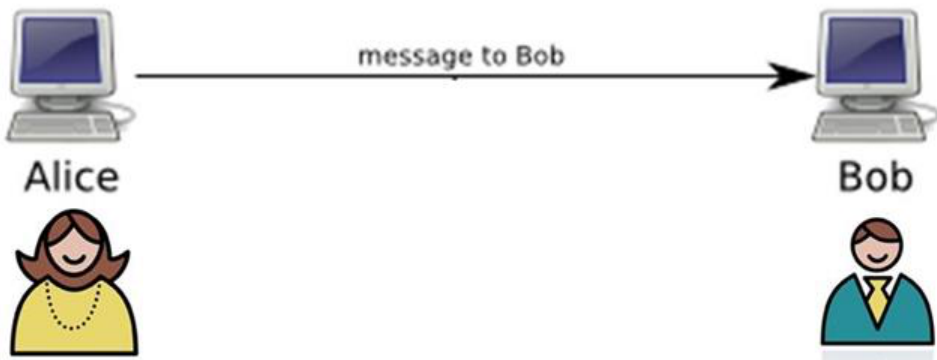
\includegraphics[width=102.48mm,height=99.20mm]{../../images/llm/page_003_img_01.png}%
\end{textblock*}

\end{document}
